\documentclass[12pt]{article}
\usepackage[margin=1in]{geometry}
\usepackage[utf8]{inputenc}
\usepackage[spanish]{babel}
\usepackage{parskip}
\usepackage{setspace}
\usepackage{amsmath}
\usepackage{graphicx}
\usepackage{hyperref} % Siempre debe ir al final.

% Opciones de Paquetes.
\decimalpoint % {babel}
\onehalfspacing % {setspace}
\graphicspath{{./img/}} % {graphicx}

% Encabezado.
\title{Clase 36. Integrales Impropias}
\author{MIT 18.01: Single Variable Calculus.}
\date{}


\begin{document}

\maketitle

\begin{abstract}
\noindent Es posible calcular integrales definidas en intervalos infinitos o con discontinuidades al interior de éstos. Se conocen como \textbf{Integrales Impropias} y, en esta clase, veremos su definición, sus tipos y cómo evaluarlas.
\end{abstract}


\section{Tasas de crecimiento y decrecimiento.}

En esta clase compararemos funciones a partir de lo rápido o lento que crecen. En la anterior también lo vimos, pero menos detallado y solo a partir de ejemplos.

Sean las funciones $f(x)$ y $g(x)$ $> 0$. A medida que $x \to \infty$, la expresión
\[
  f(x) \ll g(x)
\]
que se lee como ``$f(x)$ es muy menor a $g(x)$'', significa que:
\[
  \lim_{x \to \infty} \frac{f(x)}{g(x)} = 0
\]
Podemos usar esta notación para comparar la tasa de crecimiento de funciones conocidas a medida que $x \to \infty$. Por ejemplo, se cumple que:
\[
  \ln(x) \ll x^{P} \ll \exp(x) \ll \exp(x^{2})
\]
donde $P > 0$.

Es posible comprobar los límites entre los cuocientes de estas funciones usando la regla de L'Hôpital, puesto que todas tienden al infinito, pero al dividirlas vemos que son asintóticas en cero, lo que significa que crecen a distintas tasas como lo resumimos en la siguiente tabla:

\newpage

\begin{table}[hbt!]
\centering

\begin{tabular}{c c}
\hline
\hline
$f(x)$ & Tasa de crecimiento \\
\hline
\hline
$\ln(x)$ & Lenta \\
$x^{P}$ & Moderada \\
$\exp(x)$ & Rápida \\
$\exp(x^{2})$ & Muy rápida \\
\hline
\end{tabular}

\end{table}

También es posible evaluar a qué tasa decaen las funciones que aparecen en la tabla a medida que $x \to \infty$, por medio de sus recíprocos. Al evaluar aquello, vemos que
\[
  \frac{1}{\ln(x)} \gg \frac{1}{x^{P}} \gg \frac{1}{\exp(x)} \gg \frac{1}{\exp(x^{2})}
\]
donde $P > 0$ y la expresión $f(x) \gg g(x)$ se lee como ``$f(x)$ es mucho más grande que $g(x)$''.

Todos los recíprocos vistos arriba tienden a cero cuando $x \to \infty$, sin embargo disminuyen a distintas tasas, donde $1/\ln(x)$ es la función que lo hace más lento y $1/\exp(x^{2})$ la que lo hace más rápido. Para corroborarlo, podemos usar la regla de L'Hôpital.


\section{Integrales Impropias.}

Hasta ahora hemos calculado \textbf{integrales definidas} en intervalos finitos cerrados, donde el integrando es continuo al interior de éste. No obstante, también es posible hacerlo si uno o ambos límites son infinitos, o cuando la función que se integra tiene discontinuidades. Estos casos reciben el nombre de \textbf{Integrales Impropias}.

Las integrales impropias se dividen en \textbf{dos tipos}:

\begin{itemize}
\item \textbf{Tipo 1}: Integrales definidas con intervalos infinitos.
\item \textbf{Tipo 2}: Integrales definidas donde el integrando tiene discontinuidades en el intervalo.
\end{itemize}

Como veremos más adelante, en ambos casos calcularemos el \textbf{límite de la integral}. Según su comportamiento, señalaremos que si:

\begin{enumerate}
\item El límite es \textbf{finito} (i.e, si existe) $\rightarrow$ La integral es \textbf{convergente}.
\item El límite es \textbf{infinito} (i.e, si no existe) $\rightarrow$ La integral es \textbf{divergente}.
\end{enumerate}

\subsection{Tipo 1: Intervalos infinitos.}

Las integrales impropias de tipo 1 son aquellas donde uno o ambos de sus límites de integración son infinitos.

Sea $f(x)$ una función continua en $[a, \ \infty)$. Entonces,
\[
  \int_{a}^{\infty} f(x)dx = \lim_{b \to \infty} \int_{a}^{b} f(x)dx
\]
De igual modo, si $f(x)$ es continua en $(-\infty, \ b]$:
\[
  \int_{-\infty}^{b} f(x)dx = \lim_{a \to -\infty} \int_{a}^{b} f(x)dx
\]
Si se cumple que
\[
  \int_{a}^{\infty} f(x)dx = \lim_{b \to \infty} \int_{a}^{b} f(x)dx = L \quad \text{o} \quad
  \int_{-\infty}^{b} f(x)dx = \lim_{a \to -\infty} \int_{a}^{b} f(x)dx = L
\]
para todo número $L$, entonces decimos que las dos integrales son \textbf{convergentes}.

En cambio, si
\[
  \int_{a}^{\infty} f(x)dx = \lim_{b \to \infty} \int_{a}^{b} f(x)dx = \pm \infty \quad \text{o} \quad
  \int_{-\infty}^{b} f(x)dx = \lim_{a \to -\infty} \int_{a}^{b} f(x)dx = \pm \infty
\]
significa que ambas integrales son \textbf{divergentes}.

Cuando ambas $\int_{-\infty}^{b} f(x)dx$ y $\int_{a}^{\infty} f(x)dx$ son \textbf{convergentes}, se define que:
\[
  \int_{-\infty}^{\infty} f(x)dx = \int_{-\infty}^{c} f(x)dx + \int_{c}^{\infty} f(x)dx
\]
para todo número real $c$.

Las integrales impropias de tipo 1 se interpretan como el \textbf{área} adentro de su intervalo de integración si $f(x) \geq 0$. En ese sentido, cuando existe su límite quiere decir que el área es \textbf{finita}, mientras que es \textbf{infinita} cuando no lo hace.

\textbf{Ejemplo 1.} Sea un número cualquiera $k > 0$. Calcule la siguiente integral impropia y evalúe si converge o diverge.
\[
  \int_{0}^{\infty} \exp(-kx) dx
\]
\textbf{Solución.} Como es una integral impropia de tipo 1, comencemos estableciendo que:
\[
  \int_{0}^{\infty} \exp(-kx) dx = \lim_{b \to \infty} \int_{0}^{b} \exp(-kx) dx
\]
Luego, realicemos una sustitución directa definiendo que $u = -kx$ y, por tanto, que $du = -k dx$.
\begin{align*}
  \int_{0}^{\infty} \exp(-kx) dx &= \lim_{b \to \infty} \int_{0}^{-kb} -\frac{1}{k} \exp(u) du \\
                                 &= -\frac{1}{k} \cdot \lim_{b \to \infty} \int_{0}^{-kb} \exp(u) du \\
                                 &= -\frac{1}{k} \cdot \lim_{b \to \infty} [\exp(u)]_{0}^{-kb}
\end{align*}
Restituyamos a la variable $x$ en la antiderivada.
\begin{align*}
  \int_{0}^{\infty} \exp(-kx) dx &= -\frac{1}{k} \cdot \lim_{b \to \infty} [\exp(-kx)]_{0}^{b} \\
                                 &= -\frac{1}{k} \cdot \lim_{b \to \infty} [\exp(-kb) - \exp(-k0)] \\
                                 &= -\frac{1}{k} \cdot [\lim_{b \to \infty} \exp(-kb) - \lim_{b \to \infty} \exp(0)] \\
                                 &= -\frac{1}{k} \cdot [0 - 1] \\
  \int_{0}^{\infty} \exp(-kx) dx &= \frac{1}{k}
\end{align*}
Por lo tanto, la integral de este ejemplo es convergente en $[0, \ \infty)$, lo que significa que su área\footnote{Para $k > 0$, $\exp(-kx) > 0$ en $[0, \ \infty)$.} es finita en dicho intervalo. A continuación vemos gráficamente\footnote{En el gráfico establecí que $k = 2$.} lo que calculamos.

\begin{figure}[hbt!]
\centering
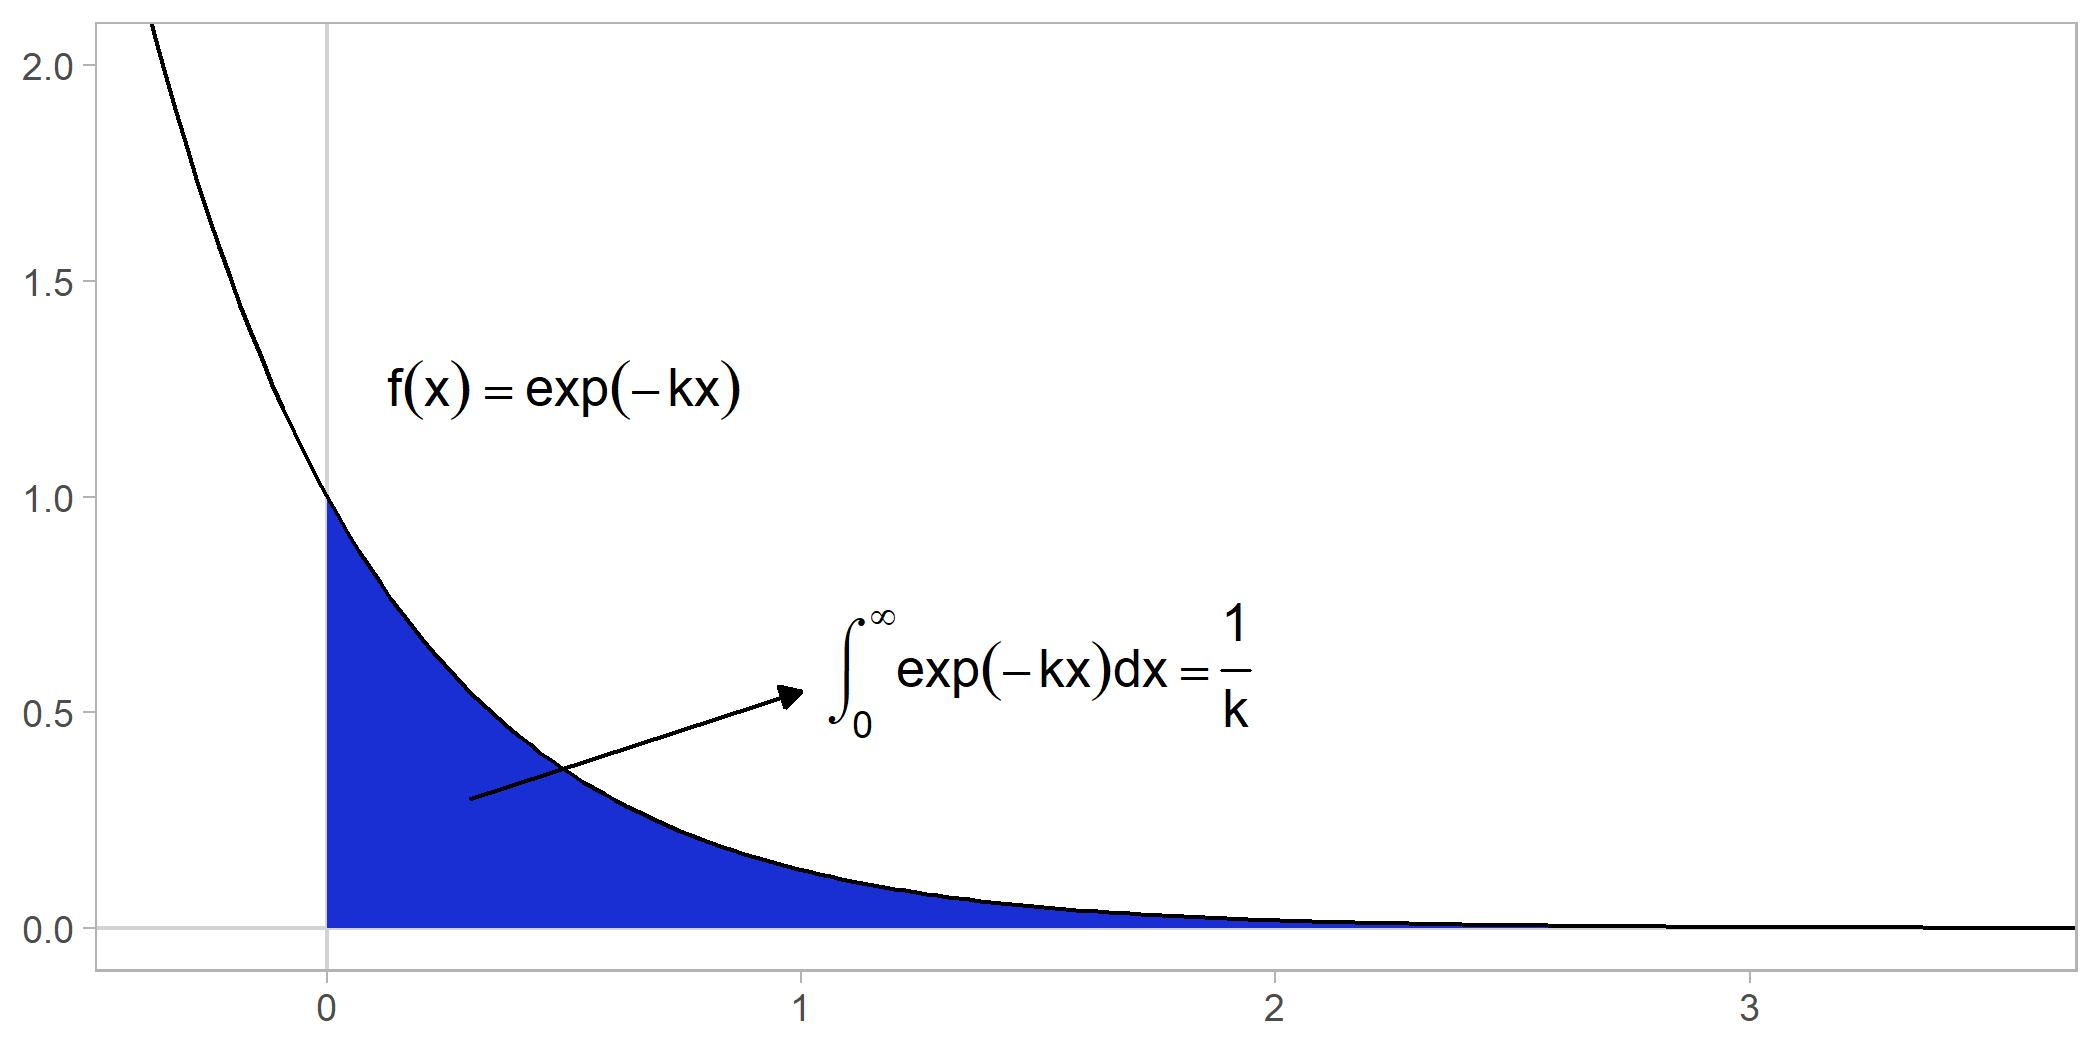
\includegraphics[scale=0.7]{example-01.jpg}
\end{figure}

\subsubsection{Evaluando el ancho de las colas de una función.}

Las integrales impropias son útiles para decidir hasta qué lugar el área bajo la curva de una función puede ser aún considerado como numéricamente relevante y cuándo ya pasa a ser un valor tan chico como para ser ignorado. Es decir, para \textbf{evaluar el ancho de su(s) cola(s)}.

Por ejemplo, en probabilidades es relevante conocer el ancho de las colas de una distribución, porque suelen esconden valores extremos o atípicos que si bien no son perceptibles visualmente, de igual modo son influyentes en los resultados generados por un modelo matemático.

Una de las distribuciones de probabilidad que se suele evaluar sus colas, es a la de forma de campana o gausiana, la cual está dada por $\exp(-x^{2})$ y que vemos a continuación.

\begin{figure}[hbt!]
\centering
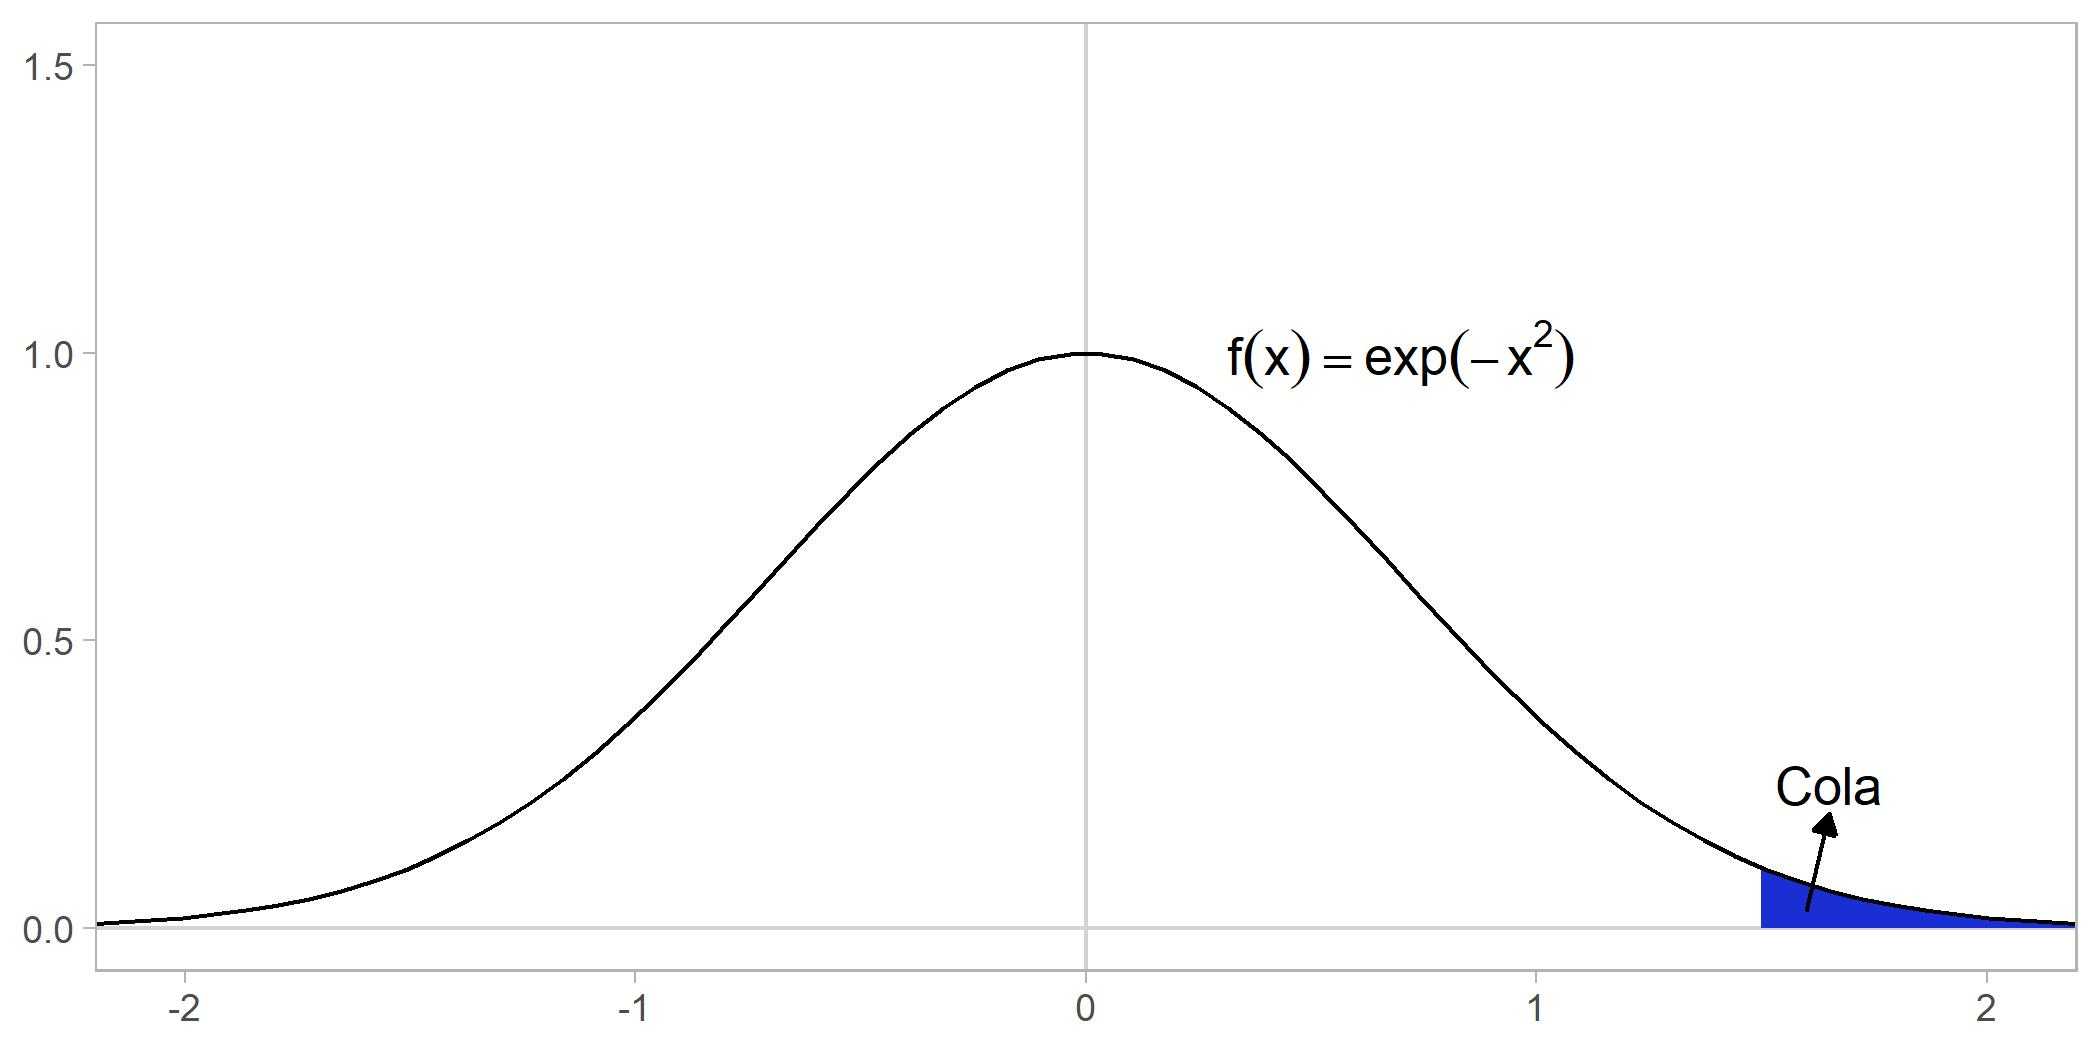
\includegraphics[scale=0.7]{bell-curve-tail.jpg}
\end{figure}

Es posible conocer numéricamente el área total de $\exp(-x^{2})$ y corresponde a\footnote{Se puede demostrar este valor a partir de una integral doble y usando coordenadas polares. Es algo que veremos en Cálculo de Varias Variables.}:
\[
  \int_{-\infty}^{\infty} \exp(-x^{2})dx = \sqrt{\pi}
\]
Ahora evaluemos la cola de otra integral impropia que sí es posible calcular analíticamente.

\textbf{Ejemplo 2.} Evalúe para cuáles valores de $P$ converge y diverge la siguiente integral:
\[
  \int_{1}^{\infty} \frac{1}{x^{P}} dx
\]

\newpage

\textbf{Solución.} Comencemos evaluando esta integral para $P = 1$.
\[
  \int_{1}^{\infty} \frac{1}{x} dx = \lim_{b \to \infty} \int_{1}^{b} \frac{1}{x} dx
                                   = \lim_{b \to \infty} [\ln(x)]_{1}^{b}
                                   = \lim_{b \to \infty} \ln(b) - \ln(1)
                                   = \infty
\]
Por lo tanto, para $P = 1$ la integral $\int_{1}^{\infty} (1/x^{P})dx$ diverge.

Ahora veámoslo para todo valor $P$, el cual es una constante.
\begin{align*}
  \int_{1}^{\infty} \frac{1}{x^{P}} dx &= \int_{1}^{\infty} x^{-P} dx \\
                                       &= \lim_{b \to \infty} \left[\frac{x^{-P + 1}}{-P + 1}\right]_{1}^{b} \\
                                       &= \lim_{b \to \infty} \frac{b^{-P + 1}}{-P + 1} - \frac{1^{-P + 1}}{-P + 1} \\
  \int_{1}^{\infty} \frac{1}{x^{P}} dx &= \lim_{b \to \infty} \left(\frac{b^{-P + 1}}{-P + 1}\right) - \frac{1}{-P + 1}
\end{align*}
Es posible observar que la antiderivada de arriba no tiene sentido para $P = 1$ porque ambas fracciones terminan con denominador igual a cero. En cambio, sí lo tiene si usamos el $\ln(x)$. En ese caso, como vimos antes, la integral diverge y no es algo aislado. Si tomamos cualquier valor $P \leq 1$ veremos que sigue el mismo comportamiento. Sin embargo, converge para $P > 1$, puesto que
\begin{align*}
  \int_{1}^{\infty} \frac{1}{x^{P}} dx &= \lim_{b \to \infty} \left(\frac{b^{-P + 1}}{-P + 1}\right) - \frac{1}{-P + 1} \\
                                       &= 0 - \frac{1}{-P + 1} \\
                                       &= \frac{-1}{-P + 1} \\
                                       &= \frac{-1}{-(P - 1)} \\
  \int_{1}^{\infty} \frac{1}{x^{P}} dx &= \frac{1}{P - 1} \qquad (\text{para } P > 1)
\end{align*}
En síntesis, este ejemplo es un caso donde podemos ver la frontera entre la divergencia y convergencia de una integral impropia. Así, podemos concluir que:

\begin{itemize}
\item Para todo $P \leq 1$, la integral $\displaystyle \int_{1}^{\infty} \frac{1}{x^{P}} dx = \infty$ (i.e, \textbf{diverge}).
\item Para todo $P > 1$, la integral $\displaystyle \int_{1}^{\infty} \frac{1}{x^{P}} dx = \frac{1}{P - 1}$ (i.e, \textbf{converge}).
\end{itemize}

A partir de lo obtenido podemos añadir que la cola derecha de $1/x^{P}$ siempre será ancha para $P \leq 1$, mientras que cuando $P > 1$ ésta irá haciéndose más angosta y, por consiguiente, podríamos evaluar en qué valores de $x$ ignoramos aquella medida al ser tan cercana a cero.

\subsection{Comparaciones directa y del límite.}

No siempre es posible evaluar integrales directamente. No obstante, en las \textbf{impropias} puede ser relevante saber si al menos \textbf{convergen o divergen}, porque si ocurre lo primero tendremos certeza que su valor será finito y podemos aproximarnos a él usando algún método numérico. En cambio, si sucede lo segundo, damos por terminado el problema.

Para evaluar si una integral no elemental converge o diverge, podemos usar los llamados criterios de \textbf{comparación directa} o de \textbf{comparación del límite}.

\subsubsection{Criterio de comparación directa.}

Supongamos que $f(x)$ y $g(x)$ son funciones continuas donde:
\[
  f(x) \geq g(x) \geq 0 \quad \text{y} \quad x \geq a
\]
Cuando se cumple lo de arriba, es posible garantizar que:

\begin{itemize}
\item Cuando $\displaystyle \int_{a}^{\infty} f(x)dx$ es \textbf{convergente}, entonces $\displaystyle \int_{a}^{\infty} g(x)dx$ es \textbf{convergente}.
\item Cuando $\displaystyle \int_{a}^{\infty} f(x)dx$ es \textbf{divergente}, entonces $\displaystyle \int_{a}^{\infty} g(x)dx$ es \textbf{divergente}.
\end{itemize}

Lo anterior se conoce como \textbf{criterio} (o teorema) \textbf{de comparación directa}.

Observemos que $f(x)$ y $g(x)$ pueden ser distintas. Esto implica que si sus integrales impropias son convergentes, no necesariamente tendrán el mismo valor, pero el principal objetivo del criterio de comparación directa es saber si dichas funciones convergen o divergen, lo que es útil cuando no es posible conocer la antiderivada de forma analítica.

\textbf{Ejemplo 3.} Evalúe si la integral es convergente o divergente.
\[
  \int_{1}^{\infty} \frac{1 + \exp(-x)}{x} dx
\]
\textbf{Solución.} Si intentamos calcular esta integral veremos eventualmente que no es elemental\footnote{Principalmente por la parte $\frac{\exp(-x)}{x}$.}. No obstante, podemos usar el criterio de comparación directa al establecer lo siguiente:
\[
  \frac{1 + \exp(-x)}{x} > \frac{1}{x}
\]
En ese sentido, podemos usar como integrando en este ejemplo a $1/x$.
\[
  \int_{1}^{\infty} \frac{1}{x} dx
\]
Y en el Ejemplo 2 vimos que para $P = 1$, la integral
\[
  \int_{1}^{\infty} \frac{1}{x^{P}} dx
\]
diverge.

Por consiguiente, es posible concluir a partir del criterio de comparación directa que la integral impropia inicial:
\[
  \int_{1}^{\infty} \frac{1 + \exp(-x)}{x} dx
\]
\textbf{diverge}.

\subsubsection{Criterio de comparación del límite.}

El otro criterio usado para evaluar integrales impropias, es el de comparación del límite.

Si las funciones $f(x)$ y $g(x)$ son positivas, continuas en $[a, \ \infty)$ y si\footnote{En la clase se señala que $L = 1$.}
\[
  \lim_{x \to \infty} \frac{f(x)}{g(x)} = L,
\]
para $0 < L < \infty$, entonces
\[
  \int_{a}^{\infty} f(x)dx \quad \text{y} \quad \int_{a}^{\infty} g(x)dx
\]
\textbf{ambas convergen o ambas divergen}.

Veamos que el límite $L$ debe ser \textbf{positivo y finito}.

\textbf{Ejemplo 4.} Evalúe la convergencia o divergencia de la integral
\[
  \int_{0}^{\infty} \frac{1}{\sqrt{x^{2} + 10}} dx
\]
\textbf{Solución.} Si bien la integral impropia de arriba es elemental, nuestro objetivo es solo evaluar su convergencia/divergencia, por tanto vamos a compararla con la integral que vemos abajo. 
\[
  \int_{1}^{\infty} \frac{1}{\sqrt{x^{2}}} dx = \int_{1}^{\infty} \frac{1}{x} dx
\]
Como vemos, cambiamos el límite inferior de la integral para evitar la discontinuidad en $x = 0$ y es posible hacerlo porque estamos evaluando si la integral original converge o diverge y no su valor exacto. Es decir, todo se mantiene intacto.

Ahora, no podemos usar el criterio de comparación directa, ya que si evaluamos los integrandos de las dos funciones dándole valores arbitrarios\footnote{Recomiendo usar valores $x \geq 1$.} a $x$, veremos que siempre:
\[
  \frac{1}{\sqrt{x^{2} + 10}} < \frac{1}{x}
\]
No obstante, podemos utilizar el criterio de comparación del límite, puesto que:
\begin{align*}
  \lim_{x \to \infty} \frac{1/\sqrt{x^{2} + 10}}{1/x} &= \lim_{x \to \infty} \frac{x}{\sqrt{x^{2} + 10}} \\
                                                      &= \lim_{x \to \infty} \frac{x \cdot (1/x)}{\sqrt{(x^{2}/x^{2}) + (10/x^{2})}} \\
                                                      &= \lim_{x \to \infty} \frac{1}{\sqrt{1 + (10/x^{2})}} \\
  \lim_{x \to \infty} \frac{1/\sqrt{x^{2} + 10}}{1/x} &= 1
\end{align*}
Usando el hecho visto en el Ejemplo 2 de que la integral
\[
  \int_{1}^{\infty} \frac{1}{x} dx
\]
diverge, por el criterio de comparación del límite podemos concluir que $\int_{0}^{\infty} \frac{1}{\sqrt{x^{2} + 10}} dx$ también \textbf{diverge}.

\subsection{Tipo 2: Integrandos con asíntotas verticales.}

Las integrales impropias de tipo 2 son aquellas donde el integrando tiene una discontinuidad en:

\begin{itemize}
\item Uno o ambos límites de integración.
\item Adentro del intervalo de integración.
\end{itemize}

A diferencia de las de tipo 1, los intervalos de las integrales impropias de tipo 2 son finitos.

Cuando la discontinuidad está en los límites del intervalo de integración, calculamos \textbf{límites laterales} de las integrales; en cambio, si está adentro de éste, dicho valor será la suma de integrales para la misma función, pero cuyos rangos limitarán donde está la asíntota vertical.

Más formalmente, sea $f(x)$ una función continua en $[a, \ b)$ y discontinua en $b$, entonces:
\[
  \int_{a}^{b} f(x)dx = \lim_{c \to b^{-}} \int_{a}^{c} f(x)dx
\]
Por otra parte, si $f(x)$ es continua en $(a, \ b]$ y discontinua en $a$, por consiguiente:
\[
  \int_{a}^{b} f(x)dx = \lim_{c \to a^{+}} \int_{c}^{b} f(x)dx
\]
Si $f(x)$ es discontinua en $c$, donde $a < c < b$, pero es continua en $[a, \ c) \cup (c, \ b]$, en consecuencia:
\[
  \int_{a}^{b} f(x)dx = \int_{a}^{c} f(x)dx + \int_{c}^{b} f(x)dx
\]
En los dos primeros casos, si los límites existen porque son finitos, señalamos que las integrales impropias son \textbf{convergentes}. Por otro lado, si los límites de éstas no existen ya que son infinitos, concluimos que son \textbf{divergentes}.

Para el tercer caso, la integral de la izquierda \textbf{converge} si las \textbf{dos integrales} que se están sumando en la derecha de la ecuación \textbf{convergen}. Si una de ellas diverge, entonces la de la izquierda también diverge.

Al igual que en las integrales impropias de tipo 1, en las de tipo 2 si $f(x) \geq 0$, podemos interpretar su valor como el área bajo la curva de esta función.

\textbf{Ejemplo 5.} Calcule la siguiente integral.
\[
  \int_{2}^{5} \frac{1}{\sqrt{x - 2}} dx
\]
\textbf{Solución.} Si bien es una integral que podemos resolver analíticamente, tenemos el problema que su integrando tiene una discontinuidad en $x = 2$ y como corresponde a su límite inferior, entonces es una integral impropia.

Para resolver esta integral impropia, podemos usar una de sus definiciones, estableciendo que:
\[
  \int_{2}^{5} \frac{1}{\sqrt{x - 2}} dx = \lim_{c \to 2^{+}} \int_{c}^{5} \frac{1}{\sqrt{x - 2}} dx
\]

Realicemos una sustitución directa a partir de $u = x - 2$ y $du = dx$.
\[
  \int_{2}^{5} \frac{1}{\sqrt{x - 2}} dx = \lim_{c \to 2^{+}} \int_{c - 2}^{3} \frac{1}{\sqrt{u}} du
                                         = \lim_{c \to 2^{+}} [2 \sqrt{u}]_{c - 2}^{3}
\]
Ahora restituyamos a la variable $x$.
\[
  \int_{2}^{5} \frac{1}{\sqrt{x - 2}} dx = \lim_{c \to 2^{+}} [2 \sqrt{x - 2}]_{c}^{5}
                                         = 2 \sqrt{3} - \lim_{c \to 2^{+}} 2 \sqrt{c - 2}
                                         = 2 \sqrt{3} - 0
                                         = 2 \sqrt{3}
\]
Por lo tanto, la integral impropia de este ejemplo es \textbf{convergente} puesto que su valor corresponde a $2 \sqrt{3}$. A continuación lo vemos de forma gráfica.

\begin{figure}[hbt!]
\centering
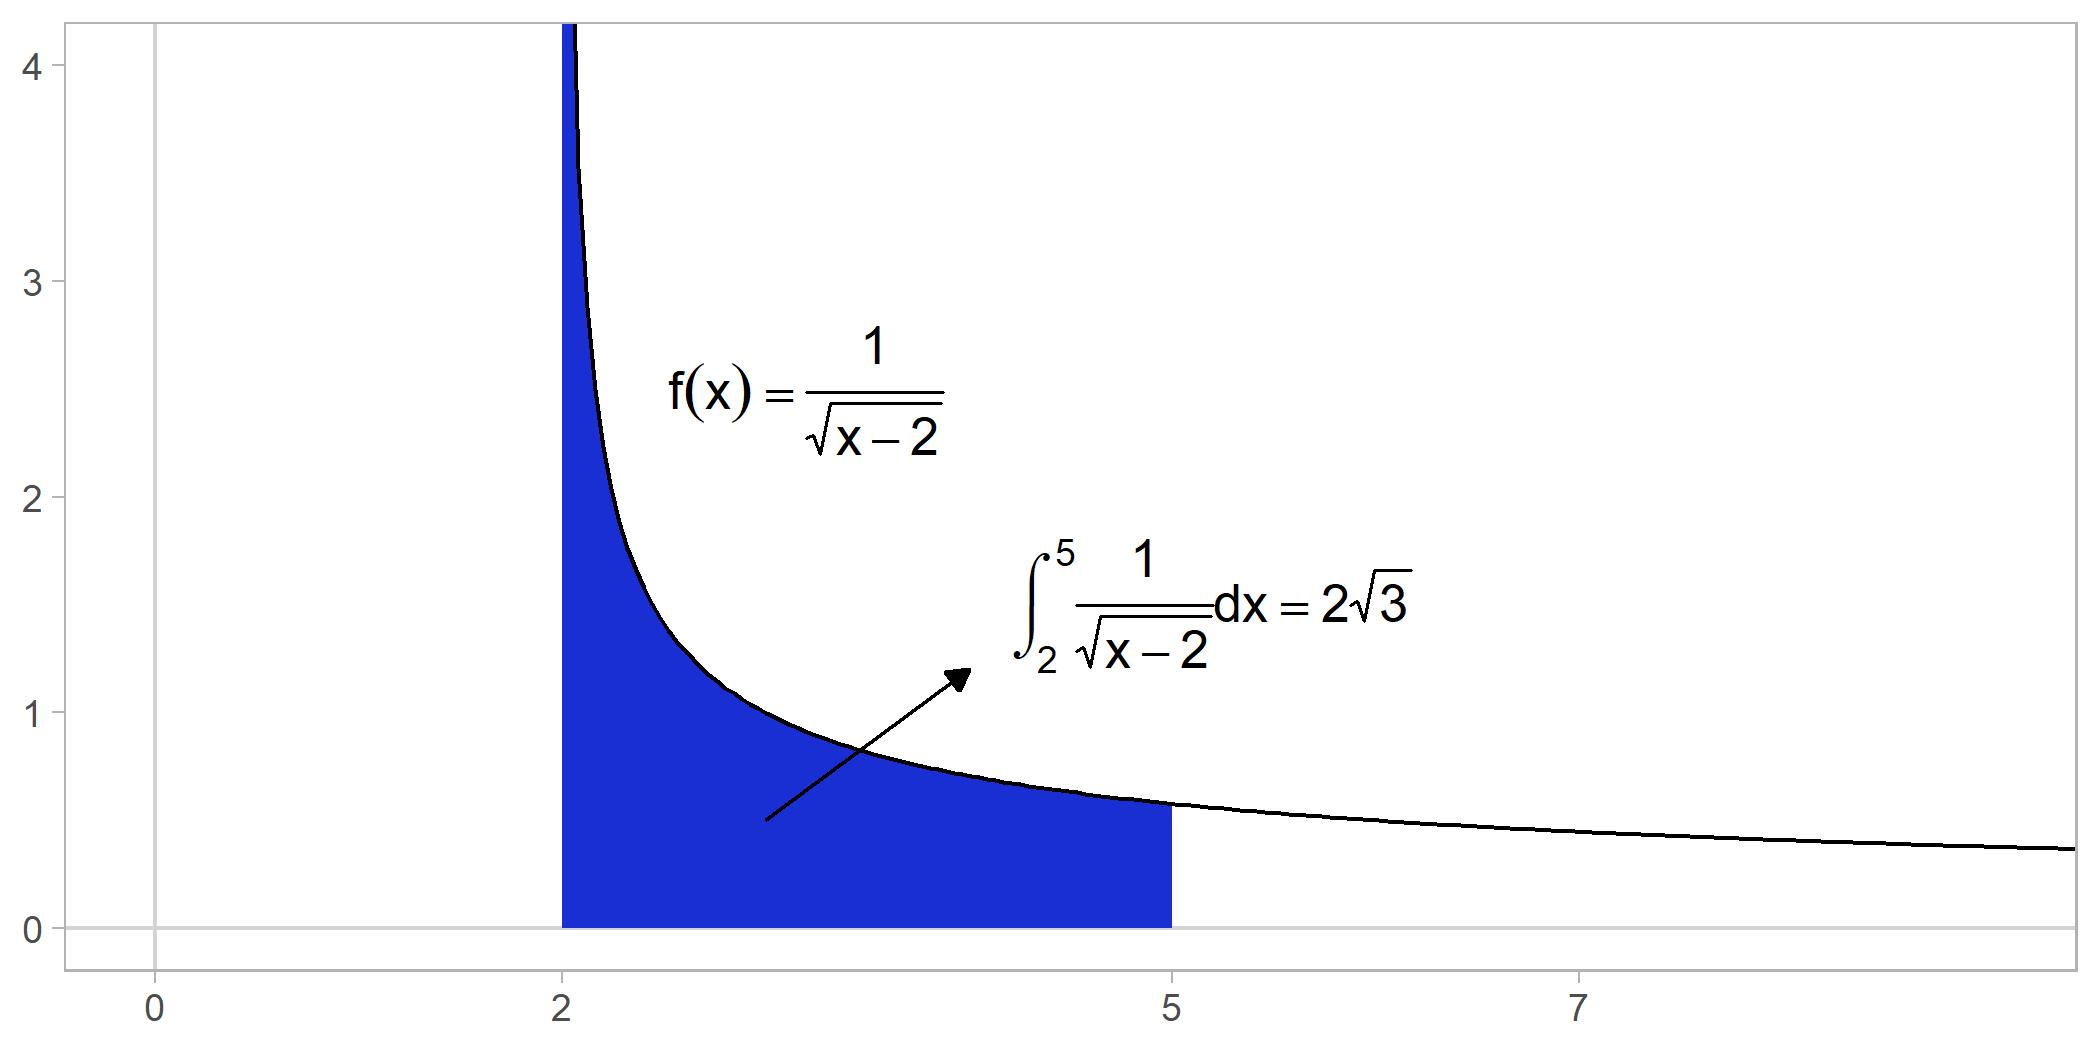
\includegraphics[scale = 0.7]{example-05.jpg}
\end{figure}

\textbf{Ejemplo 6.} Evalúe la integral
\[
  \int_{0}^{3} \frac{1}{x - 1} dx
\]
\textbf{Solución.} Esta integral debemos calcularla con mucho cuidado, puesto que si bien está definida en los límites de integración, no lo está en $x = 1$, por lo tanto corresponde a una integral impropia de tipo 2.

Como el integrando es continua en $[0, \ 1) \cup (1, \ 3]$, podemos calcular esta integral como:
\[
  \int_{0}^{3} \frac{1}{x - 1} dx = \int_{0}^{1} \frac{1}{x - 1} dx + \int_{1}^{3} \frac{1}{x - 1} dx
\]
Comencemos calculando la antiderivada del integrando de estas integrales, estableciendo que $u = x - 1$ y, por tanto, que $du = dx$.
\[
  \int \frac{1}{u} du = \ln(u) + C = \ln(x - 1) + C
\]
Lo anterior implica que:
\begin{align*}
  \int_{0}^{3} \frac{1}{x - 1} dx &= \lim_{c \to 1^{-}} [\ln(x - 1)]_{0}^{1} + \lim_{c \to 1^{+}} [\ln(x - 1)]_{1}^{3} \\
                                  &= \left[\lim_{c \to 1^{-}} \ln(c - 1) - \ln(0 - 1)\right] + \left[\ln(3 - 1) - \lim_{c \to 1^{+}} \ln(c - 1)\right] \\
                                  &= [\ln(0) - \ln(-1)] + [\ln(2) - \ln(0)] \\
                                  &= [-\infty - (-\infty)] + \infty \\
  \int_{0}^{3} \frac{1}{x - 1} dx &= -\infty
\end{align*}
En otras palabras, la integral $\int_{0}^{3} (1/(x - 1)) dx$ es \textbf{divergente}.

Acá resolvimos la suma de las integrales, pero como pudimos ver, podríamos haber concluido lo mismo con tan solo conocer una de las dos que están al lado derecho de la ecuación.




\end{document}
